%
% File acl2017.tex
%
%% Based on the style files for ACL-2015, with some improvements
%%  taken from the NAACL-2016 style
%% Based on the style files for ACL-2014, which were, in turn,
%% based on ACL-2013, ACL-2012, ACL-2011, ACL-2010, ACL-IJCNLP-2009,
%% EACL-2009, IJCNLP-2008...
%% Based on the style files for EACL 2006 by 
%%e.agirre@ehu.es or Sergi.Balari@uab.es
%% and that of ACL 08 by Joakim Nivre and Noah Smith

\documentclass[11pt,a4paper]{article}
\usepackage[hyperref]{acl2017}
\usepackage{times}
\usepackage{booktabs}
\usepackage{bbold}
\usepackage{latexsym}
\usepackage{graphicx}
\usepackage{float}
\usepackage{color}
\usepackage{multicol}
\usepackage{subcaption}
\usepackage{url}
\usepackage{etoolbox}
\usepackage{skak}
\usepackage{bm}
\usepackage{mathtools}
\newcommand{\myMatrix}[1]{\bm{\mathit{#1}}}
\usepackage[bottom]{footmisc}
\usepackage{amsmath}
\usepackage{xspace}
\usepackage{adjustbox}


\newcommand{\tabitem}{~~\llap{\textbullet}~~}
%\usepackage[draft]{hyperref}

\DeclareMathOperator{\per}{per}


\newcommand{\eqnref}[2][]{Equation#1~\ref{#2}\xspace}
\newcommand{\tabref}[2][]{Table#1~\ref{#2}\xspace}
\newcommand{\figref}[2][]{Figure#1~\ref{#2}\xspace}


%\aclfinalcopy % Uncomment this line for the final submission
%\def\aclpaperid{***} %  Enter the acl Paper ID here

%\setlength\titlebox{5cm}
% You can expand the titlebox if you need extra space
% to show all the authors. Please do not make the titlebox
% smaller than 5cm (the original size); we will check this
% in the camera-ready version and ask you to change it back.

\newcommand\BibTeX{B{\sc ib}\TeX}

\title{Joint Sentence--Document Model for Manifesto Text Analysis}

\author{First Author \\
  Affiliation / Address line 1 \\
  Affiliation / Address line 2 \\
  Affiliation / Address line 3 \\
  {\tt email@domain} \\\And
  Second Author \\
  Affiliation / Address line 1 \\
  Affiliation / Address line 2 \\
  Affiliation / Address line 3 \\
  {\tt email@domain} \\}

\date{}

\newcommand{\argmin}{\arg\!\min}
\newcommand{\norm}[1]{\vert #1 \vert}

\begin{document}


\maketitle


\begin{abstract}
Election programs (so-called manifestos) are published verbal declaration of the intentions, motives, or views of the political party. Political scientists use manifestos to understand policy-relevant themes  and also quantify a party's position on the left--right spectrum. Rather than handling the two tasks separately, we propose a joint sentence--document model for sentence-level thematic classification and document-level position quantification using manifestos in different languages. In order to handle text from multiple languages we exploit continuous neural embeddings for semantic text representation. We empirically show that the proposed joint model performs better than state-of-art approaches for the document-level task using manifestos from thirteen countries, written in six different languages.
\end{abstract}
%sentence-level
%\footnote{\url{https://en.wikipedia.org/wiki/Manifesto}} 
%Political parties are essential institutions of democracy.
% Secondly, all the works use manually coded thematic category distribution at sentence-level as features for document-level quantification task. Whereas, in this work we evaluate the effectiveness of using text for quantification task.

\section{Introduction}

% Language is the primary medium across political systems for politicians to persuade others. Though political scientists have long recognized the need for using text as data, it has not been explored due the difficulty in handling large amounts of text --- since hiring coders to manually annotate all documents was the common approach used. With automated text analysis, use of text for political data analysis is getting increased attention among political scientists \cite{ruedin2013role, gentzkow2017text}.

% Language is the medium for politics and political conflict. During election campaigns, individual candidates and political parties articulate their policy positions through party platforms and manifestos. Elected representatives debate legislation and vote for bills. After laws are passed, bureaucrats solicit comments before they issue regulations. The public discuss and express their views through social media (Twitter, blogs, Facebook), and they also launch campaigns for the change they wish to see through online petitions.  News reports document the day-to-day affairs of regional and international issues, in a way it covers information from many other sources.  It is apparent that understanding text is needed to know what political actors are speaking or writing. Though political scientists have long recognized the need for using text as data, it has not been explored due the difficulty in handling large amounts of text --- since hiring coders to manually annotate all documents was the common approach used. With automated text analysis, use of text for political data analysis is getting increased attention among political scientists \cite{ruedin2013role, gentzkow2017text}.

%Countries debate their stand on key issues in the UN. They regularly express statements that signal their priorities and also describe their motivations for cross-country ties.
%\footnote{\url{https://manifestoproject.wzb.eu/coding_schemes/mp_v5}}
%Each sentence is segmented if it discusses more than one topic and labeled.

Among many actors, political parties are at the core of contemporary democratic systems. One of the widely used datasets by political scientists is the Comparative
Manifesto Project (CMP) dataset, initiated by \newcite{CMP}, that collects party election programs (so-called manifestos) from elections in many countries around the world. The goal of the project is to provide a large data collection to support political studies on electoral processes. A sub-part of the manifestos has been manually annotated at the sentence-level with one of over fifty fine-grained political themes, divided into 7 coarse-grained topics (see \tabref{fig:CMP}).  While manual annotations are very useful for political analyses, they come with two major drawbacks. First, it is very time-consuming and labor-intensive to manually annotate each sentence with the correct category from a complex annotation scheme. Secondly, coder preferences towards particular categories might lead to annotation inconsistencies and affect comparability between manifestos annotated by different coders \cite{coder}. In order to overcome these challenges, fine and coarse-level manifesto sentence classification was addressed using supervised machine learning techniques \cite{verberne2014automatic, zirn2016classifying}. Nonetheless, manually-coded manifestos remain the crucial data source for studies in computational political science \cite{lowe2011scaling, nanni}. 
%, using a topic hierarchy defined by Dutch political experts

%  is one of the early works using manifesto text for 

% . In  authors worked with CMP dataset to do coarse-level topic classification (defined by CMP). They used Markov Logic Networks (MLN) to model sentence adjacency topic smoothness constraint. 
% --- RILE, expert survey and voter survey scores 
Other than the sentence-level labels, the manifesto text also has document-level signals,
which quantify its position on the left--right spectrum \cite{slapin2008scaling}. Though sentence-level classification and document-level quantification tasks are inter-dependent, existing work handles them separately.  We instead propose a joint sentence--document model to jointly model the two tasks. Overall, the contributions of this work are as follows:
\begin{itemize}
\item we empirically study the utility of multi-lingual embeddings for cross-lingual manifesto text analysis --- at the sentence and document-levels.

\item we evaluate the effectiveness of modelling the sentence- and document-level tasks together.

\item we study the value of \textit{country} information used in conjunction with text for the document-level regression task.
\end{itemize}


\section{Related Work}

The recent adoption of NLP methods has led to significant advances in the field of Computational Social Science \cite{lazer2009life}, including political science \cite{grimmer2013text}. Some popular tasks addressed with political text include: party position analysis \cite{biessmann2016automating};  political leaning categorization \cite{akoglu2014quantifying, zhou2011classifying}; stance classification \cite{sridhar2014collective}; identifying keywords, themes \& topics \cite{karan2016analysis, nallapati2004extraction, ding2011keyphrase}; emotion analysis \cite{rheault2016expressions}; and sentiment analysis \cite{bakliwal2013sentiment}. The source data includes manifestos, political speeches, news articles, floor debates and social media posts. 

%where the objective is to analyze large amounts of data uniformly in order to make it comparable
With the increasing availability of large-scale datasets and computational resources, large-scale comparative political text analysis has gained the attention of political scientists \cite{lucas2015computer}. For example, rather than analyzing the political manifestos of a particular party during an election, mining different manifestos across countries over time can provide deeper comparative insights into political change.

Existing classification models, except \cite{W17-2906}, utilize discrete representation of text (i.e., bag of words).  Also, most of the work analyzes manifesto text at the country level. Recent work has demonstrated the utility of neural embeddings for multi-lingual coarse-level topic classification (7 major categories) over manifesto text \cite{W17-2906}. The authors show that multi-lingual embeddings are more effective in the cross-lingual setting, where labeled data is used from multiple languages. In this work, we focus on cross-lingual fine-grained thematic classification (57 categories in total), where we have labeled data for all the languages.
%and can thus exploit only monolingual data (i.e., train and predict same language instances). Hence,

For the document-level quantification task, much work has used label count aggregation of  manually-annotated sentences as features \cite{lowe2011scaling, benoit2014putting}, while other work has used dictionary- based supervised methods, or unsupervised factor analysis based techniques \cite{hjorth2015computers, 2017arXiv170704737B}. The latter method uses discrete word representations and deals with mono-lingual text only. In \newcite{EACL}, the authors leverage neural embeddings for cross-lingual EU parliament speech text quantification with two pivot texts for extreme left and right positions. They represent the documents using word embeddings averaged with TF-IDF scores as weights. All these approaches model the sentence and document-level tasks separately.

%Rather than handling sentence and document-level tasks separately, we evaluate the utility of solving them together using joint sentence-document model under cross-lingual setting.

\section{Manifesto Text Analysis}

In the CMP, trained annotators manually label manifesto sentences according to the 57 fine-grained political categories (shown in \tabref{fig:CMP}), which are grouped into seven policy areas: External Relations, Freedom and Democracy, Political System, Economy, Welfare and Quality of Life, Fabric of Society, and Social Groups. Political parties either write their promises as a bulleted list of individual sentences, or structured as paragraphs (an example is given in \figref{fig:sub2}), proving more information on topic coherence. Also the length of documents, measured as the number of sentences, varies greatly between manifestos. The typical length (in sentences) over manifestos (948 in total) from 13 countries --- Austria, Australia, Denmark, Finland, France, Germany, Italy, Ireland, New Zealand, South Africa, Switzerland, United Kingdom and United States --- is 516.7$\pm$667. Variance in the number of sentences across documents in conjunction with class imbalance makes automated thematic classification a challenging task.  

A sentence is split into multiple segments if it discusses unrelated topics or different aspects of a larger policy, e.g. (as indicated by the different colors, and associated integer labels):
%(especially RILE quantification)
\begin{quote}
\color{red}
We need to address our close ties with our neighbours (107) \color{blue} as well as the unique challenges facing small business owners in this time of economic hardship. (402)
\end{quote}
Such examples are not common, however.\footnote{In \newcite{daubler2012natural}, based on a sample of 15 manifestos, the authors noted that around 7.7\% of sentences encode multiple topics.} Also the segmentation was shown to be inconsistent and to have no effect on quantifying the proportion of sentences discussing various topics and document-level regression tasks \cite{daubler2012natural}. Hence, consistent with previous work \cite{biessmann2016automating, W17-2906}, we consider the sentence-level classification to be a multi-class single-label problem. We use the segmented text when available (especially for evaluation), and complete sentences otherwise.
% TJB; how do you determine the label in cases of ambiguity?

A manifesto as a whole can be positioned on the left--right spectrum based on the proportion of topics discussed. We use the RILE score, which is defined as the difference between the count of sentences discussing left- and right-leaning topics \cite{cat}:
\begin{equation}
\text{RILE} = \sum_{r \in R} \per_{r} - \sum_{l \in L} \per_{l}
\end{equation}
where, $R = \{$104, 201, 203, 305, 401, 402, 407, 414, 505, 601, 603, 605, 606$\}$ and $L = \{$103, 105, 106, 107, 202, 403, 404, 406, 412, 413, 504, 506, 701$\}$, and $\per_{t}$ denotes the share of each topic $t$ as given in \tabref{fig:CMP}, per document.  Note that the RILE score is provided for almost all the manifestos in CMP dataset, but the sentence-level annotations are provided only for a subset of manifestos. That is, in some cases, the underlying annotations that the RILE score calculation was based on is often not available for a given manifesto.
%Henceforth, we use `quantification' and `regression' inter-changeably in this document.



\section{Proposed Approach}

We propose a joint sentence--document model to classify manifesto sentences into one out of 57 categories and also quantify the document-level RILE score. The joint formulation is not only to capture the task inter-dependencies, but also to use annotations at different levels of granularity (sentence and document) effectively --- a RILE score is available for 948 manifestos from 13 countries, whereas sentence-level annotations are available only for 235 manifestos. We use a neural network to model the sentence-level classification and document-level regression tasks. The proposed architecture is given in \figref{fig:HNN}. Since the text across countries is multi-lingual in nature, we use multi-lingual embeddings to represent words ($e_{w}$). We refer to the total set of manifestos available for training as $D$, and the subset which is annotated with sentence-level labels as $D_{s}$. We denote each manifesto as $d$, which has $l_{d}$ sentences $s_{1}, s_{2}, ..., s_{l_{d}}$. 

%from 13 countries ---  Austria, Australia, Denmark, Finland, France, Germany, Italy, Ireland, New Zealand, South Africa, Switzerland, United Kingdom and United States,

\begin{figure*}[!t]
\centering
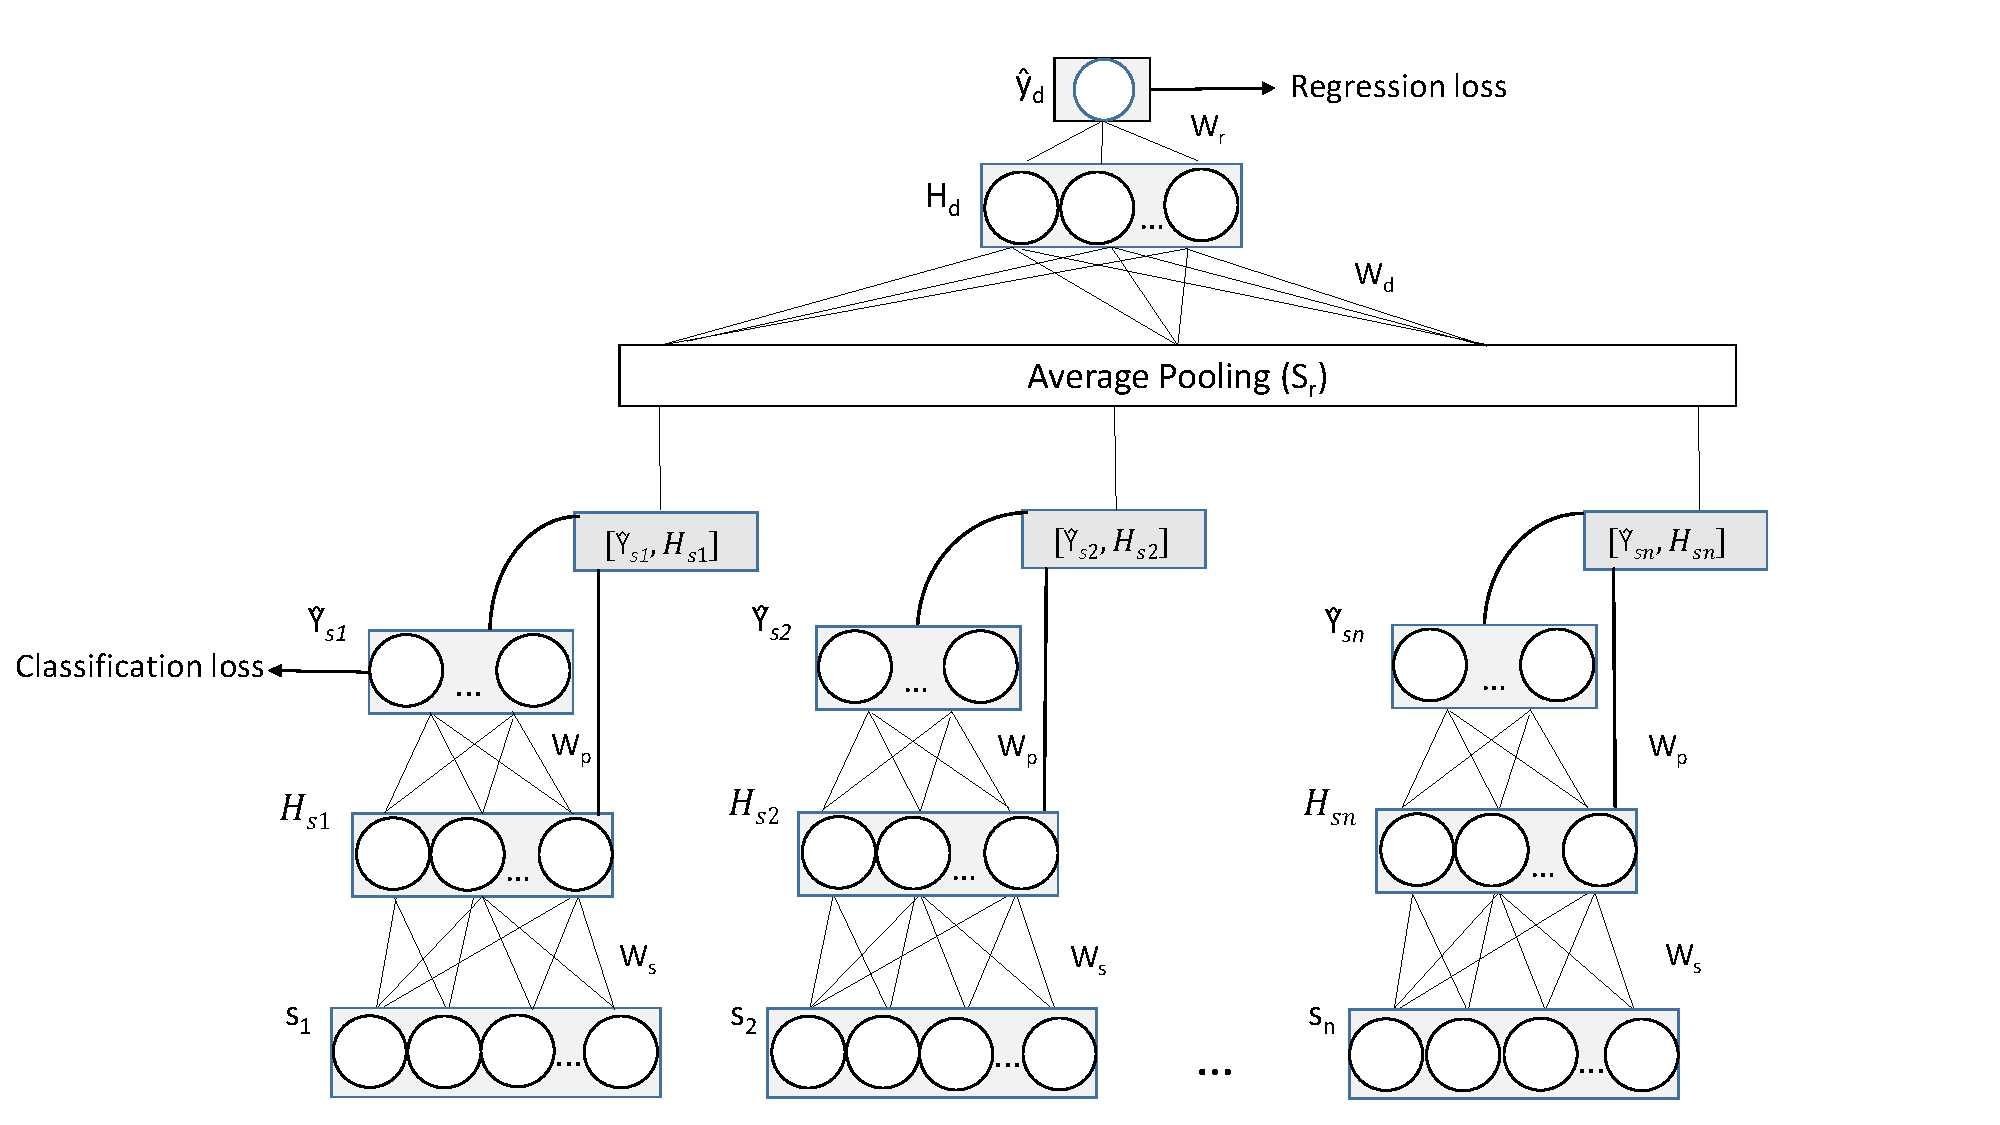
\includegraphics[height=8.4cm, scale=1.4]{ALTA_Model.pdf}
\caption{Hierarchical Neural Network for Joint Sentence--Document Analysis. $s_{1}$, $s_{2}$,...$s_{n}$ are input sentences, $W_{s}$ and $W_{p}$ are shared across unrolled sentences. $\hat{Y}_{s_{i}}$ denotes  57 classes and $\hat{y}_{d}$ denotes the estimated RILE score}
 \label{fig:HNN}
 \end{figure*}

\subsection{Sentence-level Model}
We represent each sentence using the average embedding of its constituent words, $ \bm{s}_{i} = \frac{1}{|s_{i}|}\sum_{w \in s_{i}} e_{w}$.
The average embedding representation is given as input to hidden layer with rectified linear activation units (ReLU) to get the hidden representation. Finally, the predictions are obtained using a softmax layer, which takes the hidden representation as input and gives probability of 57 classes as output.
%\[ \hat{Y}_{s_{ik}} = \frac{e^{H_{s_{i}}^\top w_{pk}}}{\sum_{j=1}^{K}{e^{H_{s_{i}}^\top w_{pj}}}}\]
% TJB: not worth defining softmax (as discussed!) ... similarly for ReLU
We use cross-entropy loss function for sentence-level model. For sentences in $D_{s}$, with ground truth labels $Y_{s}$ (one-of-K encoding), the loss function is given as follows:
  \begin{multline}
    \label{eq:sent-loss}
    L_{S}(D_{s},Y_{s})= \\
    -\frac{1}{\sum_{i=1}^{D_{s}}l_{d_{i}}}\sum_{i=1}^{D_{s}}\sum_{j=1}^{l_{d_{i}}}\sum_{k=1}^{K} Y_{s_{ijk}} \log \hat{Y}_{s_{ijk}}  
  \end{multline}
%\footnote{\url{https://keras.io/layers/wrappers/\#timedistributed}%}

\subsection{Joint Sentence--Document Model}
Using the neural network, we model the sentence-level classification and document-level regression tasks together. In the joint model, we use an unrolled (time-distributed) neural network model for the sentences in a manifesto. Here, the model minimizes cross-entropy loss for sentences over each temporal layer ($1$ to $n$). We use average-pooling with the concatenated hidden representations ($H_{s}$) and predicted output distributions ($\hat{Y}_{s}$) of individual sentences, to represent a document.\footnote{We observed that the concatenated representation performed better than using either hidden representation or output distribution.}
\begin{equation}
 S_{r} = \frac{1}{|l_{d_{i}}|}\sum_{s \in d_{i}} [\hat{Y}_{s}, H_{s}] 
\end{equation}
Since the range of RILE is $[-100,100]$, we scale it to the range $[-1,1]$ based on a final $\tanh$ layer, with $z = W_{r}^\top H_{d}$, where $H_{d}$ = ReLU$(W_{d}^\top S_{r})$, as input.
%\[ \hat{y}_{d} = \tanh(z) = \frac{e^z - e^{-z}}{e^z + e^{-z}} \]
Since it is a regression task, we minimize the mean-squared error loss function between the predicted $\hat{y}_{d}$ and actual RILE score $y_{d}$. With the given RILE scores for training documents ($Y_{d}$) and estimated scores ($\hat{Y}_{d}$), the loss function is given as follows:
%\sum_{d=1}^{D}
\begin{equation}
L_{d}(\hat{Y}_{d}, Y_{d}) = \frac{1}{|D|}  (\hat{Y}_{d} - Y_{d})^\top (\hat{Y}_{d} - Y_{d}).
\label{eq:doc-loss}
\end{equation}

Overall, the loss function for the joint model, combining \eqnref[s]{eq:sent-loss} and \ref{eq:doc-loss}, is:
\begin{equation}
 \alpha L_{s}(D_{s},Y_{s}) + (1-\alpha) L_{d}(\hat{Y}_{d}, Y_{d})
 \label{eq:joint-loss}
\end{equation}
where $0 \le \alpha \le 1$.
%\footnote{http://128.2.220.95/multilingual}
%\footnote{we use $\lambda$=1, since we give the same priority to sentence and document-level tasks} 
We evaluate both cascaded and joint training for this objective function:
\begin{description}
\item{\textbf{Cascaded Training}:} The sentence-level model is trained using $D_{s}$, to minimize $L_{s}(D_{s},Y_{s})$ in \eqnref{eq:sent-loss}, and the pre-trained model is used to obtain document-level representation $S_{r}$ for all the manifestos in training set $D$. Then the document-level regression task is trained to minimize $L_{d}(\hat{Y}_{d}, Y_{d})$ from \eqnref{eq:doc-loss}. Here, the sentence-level model parameters are fixed when the document-level regression model is trained using $S_{r}$.

\item{\textbf{Joint Training}:} As in cascaded training, the sentence-level model is pre-trained using labeled sentences. Then the entire network is updated by minimizing the joint loss function from \eqnref{eq:joint-loss}. Here the sentence-level model uses both labeled and unlabeled data.
\end{description}

%again, the sentence-level model is trained using $D_{s}$, to minimize $L_{d}(D_{s},Y_{g})$. Then
The neural network model has a single hidden layer for all the sentence and document-level approaches.  We use the Adam optimizer \cite{DBLP:journals/corr/KingmaB14} for parameter estimation. 

The proposed architecture evaluates the effectiveness of posing sentence-level topic classification as a precursor to perform document-level RILE prediction, rather than learning a model directly.  We also study the effect of the quantity of annotated text at both the sentence- and document-level for the RILE prediction task. 

%Finally, the document-level RILE score estimation can be replaced with any other task in the proposed architecture --- expert survey or voter survey scores.

%Secondly, we also study the utility of having more document-level annotations --- one-dimensional scores on the left--right spectrum, compared to sentence-level annotations, especially for sentence-level thematic classification task. 

\section{Experiments}
\subsection{Setting}
As mentioned earlier, we use manifestos collected and annotated by political scientists as part of CMP. In this work, we used 948 manifestos from 13 countries, which are written in 6 different languages --- Danish (Denmark), English (Australia, Ireland, New Zealand, South Africa, United Kingdom, United States), Finnish (Finland), French (France), German (Austria, Germany, Switzerland), and Italian (Italy). Out of the 948 manifestos, 235 are annotated with sentence level labels (from \tabref{fig:CMP}). We have RILE scores for all the 948 manifestos. Statistics about number of annotated documents and sentences across languages are given in \tabref{tab:al}.


 \begin{table}[!t]
  \centering
\begin{adjustbox}{max width=\columnwidth}
  \begin{tabular}{ c c c }
  \toprule
    Lang & \# Docs (Annotated) & \# Sents (Annotated)\\
    \midrule
    da  & 175 (36)  &  32161 (8762)	\\
    en   &  312 (94)& 227769 (73682) 	 \\    	
    fi  &  97 (16) &  18717 (8503) \\
    fr    & 53 (10) & 24596 (5559)\\
    de    & 216 (65) & 146605 (79507) \\
    it    & 95 (14)  & 40010 (4918)\\
\midrule
 Total    & 948 (235)  & 489858 (180931)\\
    \bottomrule

  \end{tabular}
  \end{adjustbox}
  \caption{Dataset statistics (da = Danish, en = English, fi = Finnish, fr = French, de = German, it = Italian).}
  \label{tab:al}
\end{table}

We use off-the-shelf multi-lingual word embeddings\footnote{\url{http://128.2.220.95/multilingual}} to represent words. We chose embeddings trained using translation invariance approach \cite{ammar2016massively}, with dimensionality 512, since we found it to perform better than other approaches. 

\subsection{Sentence-Level Classification}
We first compare traditional bag-of-words discrete representation with distributed neural representation for words for fine-grained thematic classification, under mono-lingual training setting (\em{Mono-lingual}). \rm Hence we compare the following approaches. 
%Following are the sentence classification baseline techniques that we compare our proposed approach against.

\begin{description}
\item{Bag of words (\em{BoW-LR}, \em{BoW-NN}):} We use TF-IDF representation for sentences and build a model for each language separately. We use Logistic Regression classifier, which is the state-of-art approach for fine-grained manifesto sentence classification \cite{biessmann2016automating}. We refer to this approach as \em{BoW-LR}. \rm We also use Neural Network classifier, which we refer as \em{BoW-NN}. \rm

\item{Language-wise average embedding (\em{AE-NN$_{m}$}):} \rm We build a Neural Network classifier per language, with average neural embedding as sentence representation.
\end{description}

% Commonly for all empirical evaluation, we compute micro-average performance with 80-20\% train-test ratio across 10 runs with random split (at document-level), where the 80\% split also contains sentence-level annotated documents proportionally.  We compute micro-averaged F-score\footnote{Harmonic mean of precision and recall, \url{https://en.wikipedia.org/wiki/F1_score}} to evaluate sentence classification performance. In the mono-lingual setting (\tabref{tab:res1}), using word embeddings provides better performance compared to bag-of-words for en, fi, de and it. 

% \begin{table}[!htp]
%   \centering
%   \begin{tabular}{ c c c c}
%   \toprule
%     Lang. & BoW-LR & BoW-NN & LWE-NN \\
%     \midrule
%     da  & 	0.29 & \textbf{0.36} & 0.24\\
%     en   &  0.24 & 0.29 & \textbf{0.43}\\    	
%     fi  &   0.21 & 0.23 & \textbf{0.26}\\
%     fr    & 0.28 & \textbf{0.28} & 0.24\\
%     de    &  0.20 & 0.23 & \textbf{0.31}\\
%     it    & 0.14 & 0.22 & \textbf{0.25} \\
% \midrule
% Avg.    & 0.22 & 0.26 & 0.35\\
%     \bottomrule

%   \end{tabular}
%   \caption{Micro-Averaged F-measure. Best scores are given in bold under each language setting}
%   \label{tab:res1}
% \end{table}
Since distributed representation allows to leverage text across languages, we evaluate the following approaches with combined training sentences across languages (\em{Cross-lingual}). \rm

\begin{description}
\item{Convolutional Neural Network (\em{CNN}):} CNN was shown to be effective for cross-lingual manifesto text coarse-level (7 major domains as shown in \tabref{fig:CMP}) topic classification \cite{W17-2906}. So, we evaluate CNN with a similar architecture --- single convolution layer (32 filters with window size 3), followed by single max pooling layer and finally a softmax layer. We use neural embeddings to represent words.
\item{Combined average embedding (\em{AE-NN$_{c}$}):} We build a Neural Network classifier with training instances combined across languages, with average neural embedding as sentence representation. This is our proposed approach for sentence-level model.
\end{description}

Commonly for all empirical evaluation, we compute micro-averaged performance with 80-20\% train-test ratio across 10 runs with random split (at document level), where the 80\% split also contains sentence level annotated documents proportionally. Optimal model parameters we found for the proposed model (\figref{fig:HNN}) are $\norm{H_{s}}$ = 300, $\norm{H_{d}}$ = 10. We compute F-score\footnote{Harmonic mean of precision and recall, \url{https://en.wikipedia.org/wiki/F1_score}} to evaluate sentence classification performance. Sentence classification performance is given in \tabref{tab:alx}. In the mono-lingual setting (\tabref{tab:alx}), using word embeddings did not provide better performance compared to bag-of-words. (except for $en$ which was the source language for obtaining multi-lingual embeddings). 

Under cross-lingual setting, \em{AE-N$N_{c}$} \rm is the sentence-level Neural Network model. We use \em{AE-N$N_{c}$} \rm in the \textit{cascaded training} for obtaining document-level RILE prediction. Note that in \textit{cascaded training}, sentence and document-level models are trained separately in a cascaded fashion. Joint-training results where the sentence model is trained in a semi-supervised way together with document-level regression task is referred to as \em{JT$_{s}$}\rm. We set  $\alpha$=0.4 (in equation (4)) empirically which gave the best score for both sentence and document-level tasks. We observed a trade-off in performance with different $\alpha$, with lesser $\alpha$ (0.1), document-level correlation increases (to 0.52) while sentence-level F-score decreases (to 0.33). Higher value of $\alpha$ (0.9) gives performance closer to cascaded training. \em{JT$_{s}$} \rm has a comparable performance with \em{AE-NN$_{c}$}. \rm It must be considered that the (sentence and document-level) model built using cascaded training is a special case of jointly trained model, with suitable values of $\alpha$ (closer to 1). Also \em{CNN}, \em{AE-NN}$_{c}$ and \em{JT}$_{s}$ \rm use combined training instances across languages compared to other approaches. Except for $da$ and $it$ cross-lingual training performs better than mono-lingual setting. Overall, the proposed approach shows slight improvement over baseline approaches for sentence classification task.
%Also \textit{CNN}, $AE$-$NN_{c}$ and \textit{$JT_{s}$} use combined training instances across languages compared to other approaches.
%Hence other than en and de which have sufficient labeled data, models that use combined training data perform better. %Since the number of documents are not many compared to sentences, joint training 
%\clearpage

 \begin{table*}[!htp]
  \centering
  %\begin{tabular}{ c | c c c | c c c}
  \begin{tabular}{ c@{\hskip 0.2in} c c c@{\hskip 0.25in} c c c}
  \toprule
   &  \multicolumn{3}{c}{Mono-lingual} & \multicolumn{3}{c}{Cross-lingual} \\
  \toprule
    \em{Lang.} & \em{BoW-LR} & \em{BoW-NN} & \em{AE-NN}$_{m}$ & \em{CNN} & \em{AE-NN}$_{c}$ & \em{JT}$_{s}$\\
    \midrule
    da  & 	0.29 & \textbf{0.35} & 0.24 & 0.30 & 0.28 & 0.30\\
    en   &  0.36 & 0.38 & \textbf{0.42} & 0.40 & \textbf{0.42} & 0.41\\    	
    fi  &   0.21 & 0.29 & 0.26 & \textbf{0.30} & 0.27 & 0.26\\
    fr    & 0.28 & 0.36 & 0.24 & 0.36 & 0.37 & \textbf{0.38} \\
    de    &  0.30 & 0.31 & 0.31 & 0.31 & 0.31 & \textbf{0.33}\\
    it    & 0.32 & \textbf{0.33} & 0.25 & 0.30 & 0.32 & 0.26\\
\midrule
Avg.    & 0.32 & 0.34 & 0.35 & 0.34 & \textbf{0.36} & 0.35\\
%\midrule

 \bottomrule

  \end{tabular}
  \caption{Micro-Averaged F-measure. Best scores are given in bold under each language setting}
  \label{tab:alx}
\end{table*}

\subsection{Document-Level Regression}
For document-level regression task, following are the baseline approaches. Note that we use $\tanh$ output for all the models, since the range of re-scaled RILE is from -1 to +1.

% with \textit{tanh} output.
\begin{description}
\item{Bag of words (\em{BoW-NN$_{d}$}):} \rm We use TF-IDF representation for documents and build a Neural Network model  for each language.
%(to capture non-linear patterns)
%regression model for each country and language separately. We use Linear Regression; referred to as \textit{LR-CTR} and \textit{LR-Lang} which are models built per country and language respectively. Since language-wise model performed better than country-wise model, we also build a
\item{Average embedding (\em{AE-NN}$_{d}$):} We use average embedding of words in the document to build a Neural Network model across languages.

\item{Bag-of-Centroids (\em{BoC}):} Here the word embeddings are clustered into $K$ different clusters using K-Means clustering algorithm, and  words in each document are assigned to clusters based on its euclidean-distance ($dist$) to cluster-centroids ($C$). 
\[ cluster (word) = \argmin_k dist(C_{k}, word) \]
Finally, each document is represented by the distribution of words mapped to different clusters (1 X $K$ vector). We use a Neural Network regression model with bag-of-centroids representation. Results with $K$=1000, which performed best is given in Table 3.

\item{sentence-level model and RILE formulation (\em{AE-NN}$_{c}^{rile}$)}: Here the predictions of sentence-level model (\em{AE-NN$_{c}$}) \rm are used directly with RILE formulation (equation (1)) to derive RILE score for manifestos.

\item{Cross-lingual scaling (\em{CLS}):} This is a recent unsupervised approach for cross-lingual political speech text positioning task \cite{EACL}. Authors use average word-embeddings weighed by TF-IDF score to represent documents.\footnote{We use this aggregate representation since it was shown to be better than word alignment and scoring approach \cite{EACL}} Then a graph is constructed using pair-wise distance of documents. Given two pivots texts for extreme left and right positions [-1, +1], label propagation approach is used to quantify other documents in the graph.
\end{description}

 \begin{table}[!t]
  \centering
  \begin{tabular}{ c c c }
  \toprule
    Approach & MSE($\downarrow$) & $r(\uparrow)$\\
    \midrule
    %LR-CTR  & 	0.874 & 0.18 \\
    %LR-Lang   &  0.684 & 0.24\\    	
    \em{BoW-NN}$_{d}$  &   0.054 & 0.23\\
    \em{AE-NN}$_{d}$    & 0.057 & 0.14\\
    \em{BoC}    &  0.052 & 0.33\\
    \em{AE-NN}$_{c}^{rile}$   & 0.060 & 0.35\\
    %CLS   & 0.815 & 0.24\\
    \em{CLS}   & -- & 0.24\\
    \em{Cas}$_{d}$  &  0.050 & 0.41 \\
    \em{JT}$_{d}$ &  \textbf{0.044} & \textbf{0.47} \\
    \bottomrule
  \end{tabular}
  \caption{RILE score prediction performance. Best scores are given in bold %CLS assigns -1 and +1 for extreme manifestos and propagates the values on a graph. Since they solve it as a classification problem, MSE is not applicable. 
(higher is better for $r$, and lower is better for MSE).}
  \label{tab:al1}
\end{table}

RILE score regression performance results are given in \tabref{tab:al1}. Other than \em{BoW-NN$_{d}$} \rm all other approaches are cross-lingual. We evaluate document-level performance using mean-squared-error (MSE) and Pearson correlation ($r$). The proposed approach's performance, using cascaded training  is referred to as \em{Cas}$_{d}$ \rm and jointly trained model is referred to as \em{JT}$_{d}$. \rm Overall the jointly trained model performs best for document-level task, with a comparable performance at sentence-level task. 

% \subsection{Joint Training}
% Here we provide results for the joint model, where the sentence model is trained in a semi-supervised way together with document-level regression task. We observed that the jointly trained model did not perform better than cascaded model fine-tuned for document-level task.

\subsection{Quantity of Annotation}
We measure the importance of annotated text at sentence and document-level for RILE score regression task. We vary the percentage of labeled data, while keeping the test sample size at 20\% as before. In the first setting, we keep the training ratio of documents at 80\%, within that 80\% we increase the proportion of documents with sentence-level annotations --- from 0 (document average embedding setting, \em{AE-NN}$_{d}$) \rm to 80\%. Results are given in \figref{fig:sentl}. Similarly, in the other setting, we keep the training set with 80\% sentence-level annotated documents (which is $\sim$20\% of the total data), and add documents (with only RILE score), increasing the training set from 20 to 80\%. Results of this study are given in \figref{fig:docl}. We observed that, jointly-trained model uses sentence-level annotations more effectively than cascaded approach (\figref{fig:sentl}) --- even with less sentence-level annotations. Also, with less document-level signal (up to 40\%) for training, both the approaches perform similarly ($r$). As the training ratio increases, joint-training leverages both sentence and document-level signals effectively.


\begin{figure}[!t]
\centering
  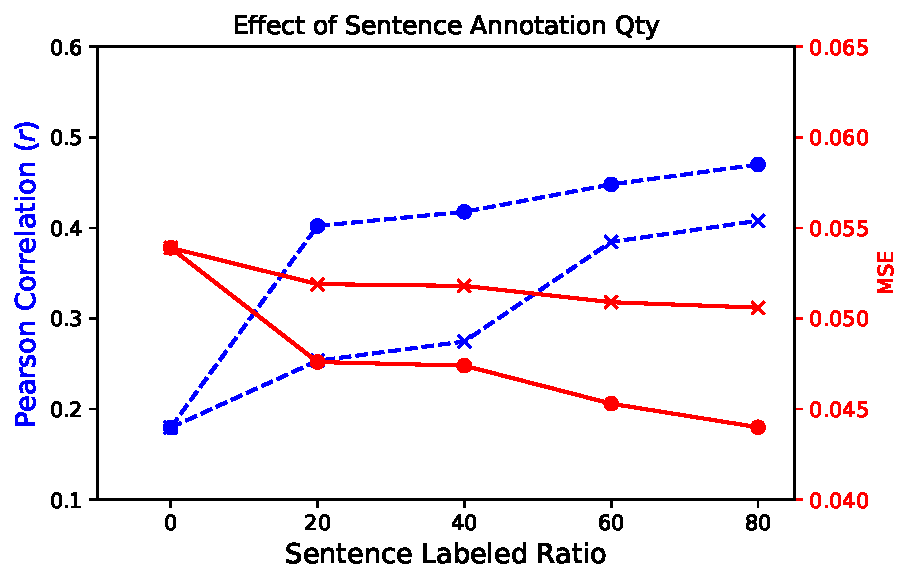
\includegraphics[width=0.92\linewidth]{altw1.pdf}
  \caption{Fixing 80\% training documents with RILE score, ratio of documents with sentence-level annotations is varied. \begin{small} $\markera$ \end{small} denotes \em{Cas}$_{d}$ \rm and \begin{small} $\markerb$ \end{small} denotes \em{JT}$_{d}$}
  \label{fig:sentl}
\end{figure}

\begin{figure}[!t]
\centering
  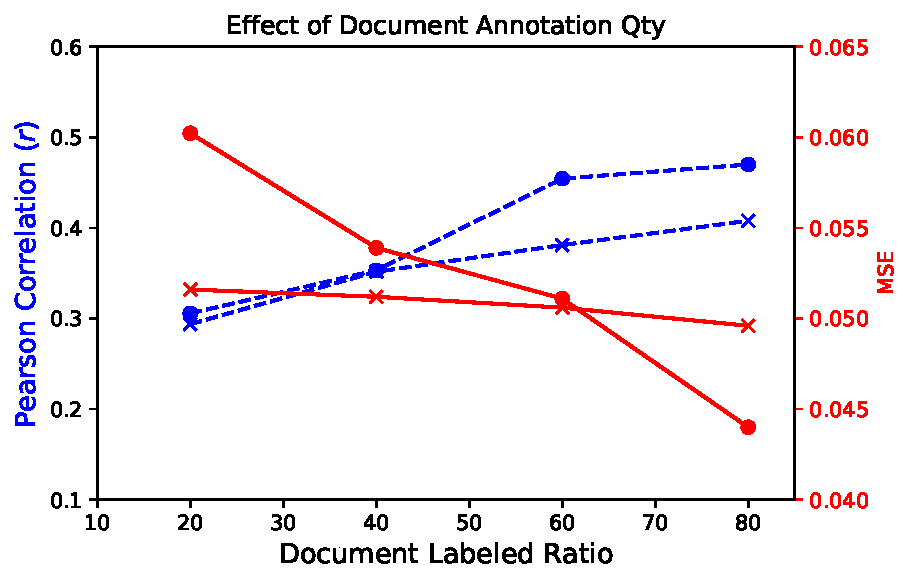
\includegraphics[width=0.92\linewidth]{altw2.pdf}
  \caption{Fixing 80\% training documents with sentence-level annotations, ratio of documents with RILE score is varied. \begin{small} $\markera$ \end{small} denotes \em{Cas}$_{d}$ \rm and \begin{small} $\markerb$ \end{small} denotes \em{JT}$_{d}$}
 \label{fig:docl}
 \end{figure}
 
\subsection{Use of Country Information}
Since the definition of left--right varies between countries, we study the influence of \textit{country} information in the proposed model with \textit{joint-training}. We use two ways to incorporate country information \cite{hoang2016incorporating}: (a) \textit{stack} --- one-hot encoding (13 countries, 1 X 13 vector) of each manifesto's \textit{country} is concatenated with hidden representation of the document ($S_{r}$ in \figref{fig:HNN}) (b) \textit{non-linear stack} --- one-hot-encoded country vector is passed through a hidden layer with $\tanh$ non-linear activation and concatenated with $S_{r}$. With both the models we observed mild improvement in correlation (given in \tabref{tab:al2}).

 \begin{table}[t!]
  \centering
  \begin{tabular}{ c c c }
  \toprule
    Approach & MSE & $r$\\
    \midrule
    stack &  0.045 (0.001 $\downarrow$) & 0.49 (0.02 $\uparrow$) \\
    non-linear stack &  0.048 (0.004 $\downarrow$) & 0.48 (0.01 $\uparrow$) \\
    \bottomrule
  \end{tabular}
  \caption{RILE score prediction performance with \textit{country} information. Difference compared to $JT_{d}$ is given within paranthesis. $\uparrow$ -- improvement, $\downarrow$ -- decrease in performance}
  \label{tab:al2}
\end{table}

\section{Conclusion and Future Work}
In this work we evaluated the utility of a joint sentence--document model for sentence-level thematic classification and document-level RILE score regression tasks. Our observations are as follows: (a) joint model performs better than state-of-art approaches, where cascaded training can be seen as a special case of joint training. (b) joint-training leverages sentence-level annotations more effectively than cascaded approach for RILE score regression task. There are many extensions possible to the current work. First is to handle class imbalance in the dataset with a cost-sensitive objective function. Secondly, CNN gave a comparable performance with Multi-layer Perceptron (NN), which motivates the need to evaluate an end-end sequential architecture. Off-the-shelf embeddings leads to out-of-vocabulary scenarios. It could be beneficial to  adapt word-embeddings with manifesto corpus. Finally, background information such as country can be leveraged more effectively.

%We used off-the-shelf embeddings, which leads to out-of-vocabulary scenarios. It could be beneficial to  adapt word-embeddings with manifesto corpus.

\begin{figure*}[t!]
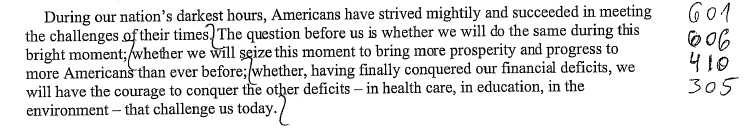
\includegraphics[width=1\linewidth]{US_Democrats_1.png}
\caption{Democratic Party of USA, 2000 --- $\int$ denotes sentence segment. 601 = National Way of Life: Positive, 606 = Civic Mindedness: Positive, 410 = Economic Growth: Positive, 305 = Political Authority}
\label{fig:sub2}
\end{figure*}

% \begin{figure*}[!ht]
% \centering
% \begin{subfigure}{.45\textwidth}
%   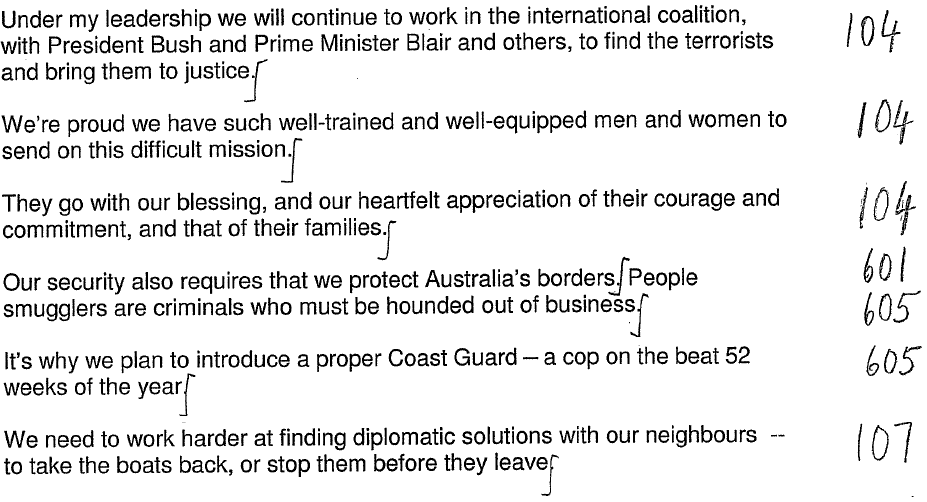
\includegraphics[width=1\linewidth]{Aus_Labor.png}
%   \caption{Australian Labor Party, 2001}
%   \label{fig:sub1}
% \end{subfigure}%
% \begin{subfigure}{.55\textwidth}
%   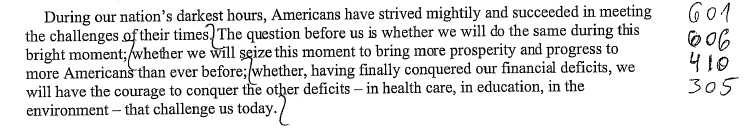
\includegraphics[width=1.1\linewidth]{US_Democrats_1.png}
%   \caption{Democratic Party of USA, 2000}
%   \label{fig:sub2}
%  \end{subfigure}
%  \caption{Sample Manifestos --- $\int$ denotes sentence segment}
%  \end{figure*}

\begin{small}
\begin{table*}
  %\centering
  \begin{tabular}{lll}
    \toprule
    \multicolumn{2}{c}{\begin{centering} \textbf{CMP Coding Scheme}\end{centering}} \\[.5\normalbaselineskip]
 %   Types & Type of Critical Point & Stability \\
    \midrule
   \tabitem Domain 1.~External Relations  & 411 Technology and Infrastructure: Positive\\
   	101 Foreign Special Relationships: Positive & \color{red} 412 Controlled Economy\\
    102 Foreign Special Relationships: Negative & \color{red} 413 Nationalisation\\
  \color{red}  103 Anti-Imperialism & \color{blue} 414 Economic Orthodoxy\\
  \color{blue}  104 Military: Positive & 415 Marxist Analysis \\
 \color{red}   105 Military: Negative & 416 Anti-Growth Economy: Positive \\
   \color{red} 106 Peace & \\
   \color{red} 107 Internationalism: Positive & \tabitem Domain 5: Welfare and Quality of Life \\
    108 European Community/Union: Positive & 501 Environmental Protection\\
    109 Internationalism: Negative &   502 Culture: Positive\\
    110 European Community/Union: Negative & 503 Equality: Positive\\
     &  \color{red} 504 Welfare State Expansion\\
   \tabitem Domain 2: Freedom and Democracy &  \color{blue}   505 Welfare State Limitation\\
  \color{blue} 201 Freedom and Human Rights & \color{red} 506 Education Expansion\\
 \color{red} 202 Democracy & 507 Education Limitation\\
  \color{blue} 203 Constitutionalism: Positive \\
  204 Constitutionalism: Negative & \tabitem Domain 6: Fabric of Society\\
    & \color{blue} 601 National Way of Life: Positive\\
\tabitem Domain 3: Political System &    602 National Way of Life: Negative
\\
  301 Decentralisation & \color{blue}  603 Traditional Morality: Positive
\\
  302 Centralisation &   604 Traditional Morality: Negative
\\
  303 Governmental and Administrative Efficiency &  \color{blue}  605 Law and Order: Positive
\\
  304 Political Corruption &  \color{blue} 606 Civic Mindedness: Positive
\\
  \color{blue} 305 Political Authority &   607 Multiculturalism: Positive
\\
&   608 Multiculturalism: Negative\\
\tabitem Domain 4: Economy  & \\
 \color{blue} 401 Free Market Economy & \tabitem Domain 7: Social Groups\\
 \color{blue} 402 Incentives: Positive & \color{red} 701 Labour Groups: Positive\\
\color{red}  403 Market Regulation & 702 Labour Groups: Negative\\
\color{red}  404 Economic Planning & 703 Agriculture and Farmers: Positive\\
  405 Corporatism/Mixed Economy & 704 Middle Class and Professional Groups\\
\color{red}  406 Protectionism: Positive & 705 Underprivileged Minority Groups\\
\color{blue}  407 Protectionism: Negative & 706 Non-economic Demographic Groups\\
  408 Economic Goals & \\
  409 Keynesian Demand Management & \\
  410 Economic Growth: Positive & 000 No meaningful category applies\\
    \bottomrule   
  \end{tabular}
  \caption{\textit{Left} topics are given in \textit{\color{red}red} and \textit{right} topics are given in \textit{\color{blue}blue}}
  \label{fig:CMP}
\end{table*}
\end{small}
% \begin{figure*}[!ht]
% \centering
% 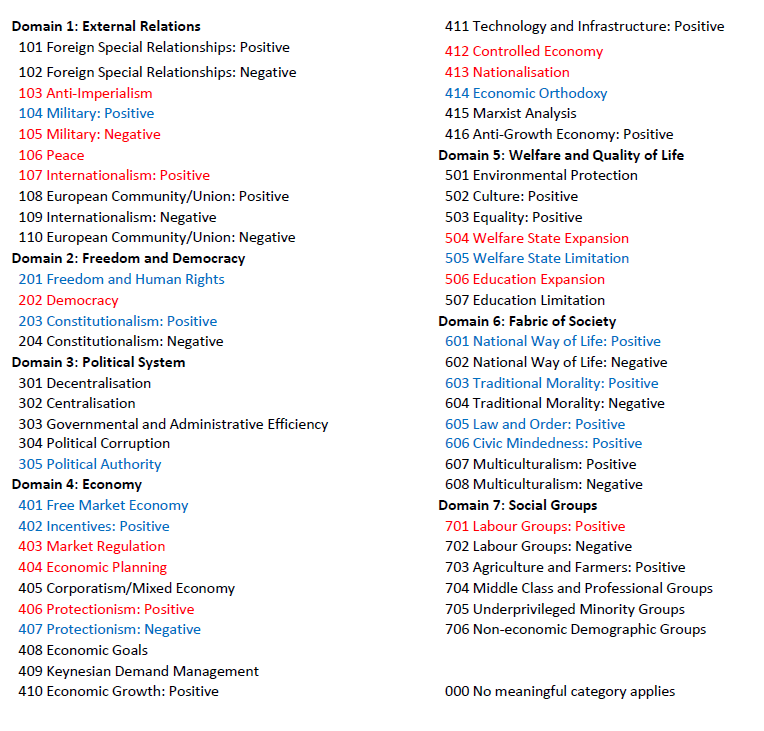
\includegraphics[width=1\linewidth]{CMP_Coding_1.png}
% \caption{\textit{Left} topics are given in red, \textit{right} topics are given in blue and the rest are given in black}
% \label{fig:CMP}
% \end{figure*}

\bibliography{acl2017}
\bibliographystyle{acl_natbib}

%\section{Appendix}



% \begin{figure*}[ht]
% \centering
% \begin{subfigure}{.45\textwidth}
%   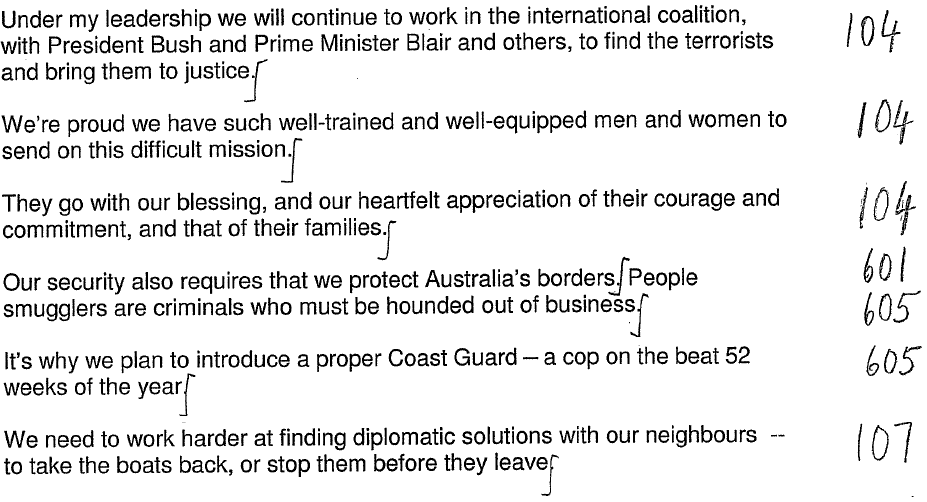
\includegraphics[width=1\linewidth]{Aus_Labor.png}
%   \caption{Australian Labor Party, 2001}
%   \label{fig:sub1}
% \end{subfigure}%
% \begin{subfigure}{.55\textwidth}
%   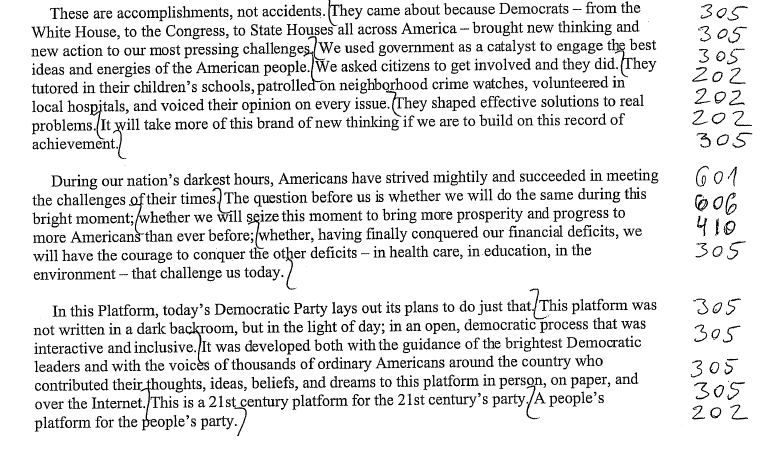
\includegraphics[width=1\linewidth]{US_Democrats.png}
%   \caption{Democratic Party of USA, 2000}
%   \label{fig:sub2}
%  \end{subfigure}
%   \begin{subfigure}{.6\textwidth}
%   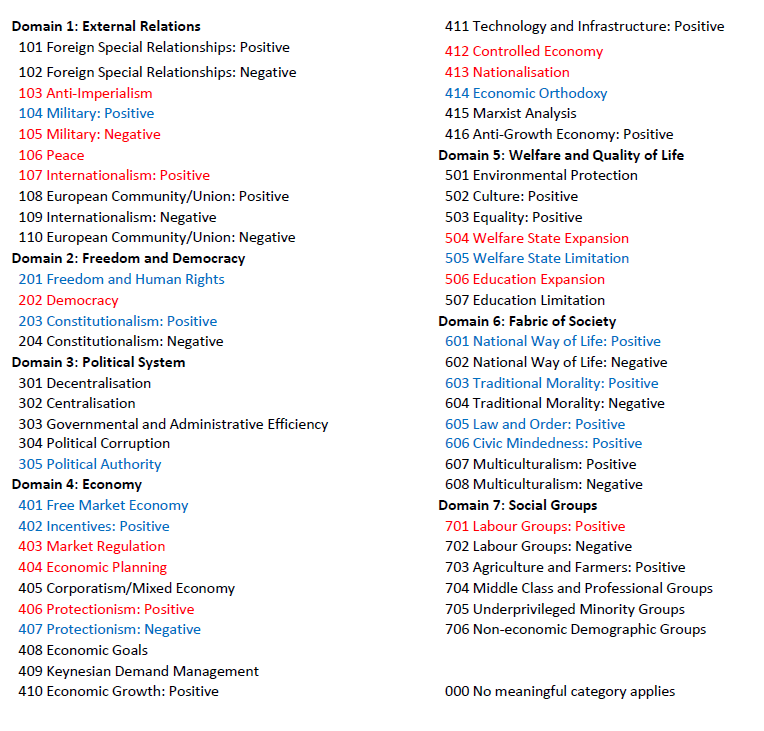
\includegraphics[width=1.3\linewidth]{CMP_Coding_1.png}
%   \caption{\textit{Left} topics are given in red, \textit{right} topics are given in blue and the rest are given in black}
%   \end{subfigure}
% \caption{Sample Manifestos (a and b) and CMP coding scheme (c)}
% \label{fig:test}
%  \end{figure*}
 
\end{document}

%%% Local Variables:
%%% mode: latex
%%% TeX-master: t
%%% End:
